\section{CanOp}
CanOp est le nom qui a été donnée au projet de crée une sonde nouvelle generation pour la mine Somaïr au Niger. Cette sonde est composer de 3 piece 
\begin{itemize}
    \item 2 Sonde de rayonement Gamma fournit par la societer Geovista
    \item Une partie elctonique qui inclue une batterie.
    \item Un GPS differentielle fournit par Ophelia 
\end{itemize}
Un operateur Utilise cette sonde en conjection avec une tablette pour determiner ou extraire du minerai. 
\subsection{Les sonde Gamma}
\label{ssec:sonde}
Les sonde gamma de cette appariel provienne de chez ophelia et sont composer de deux partie.
\begin{figure}
    \centering
    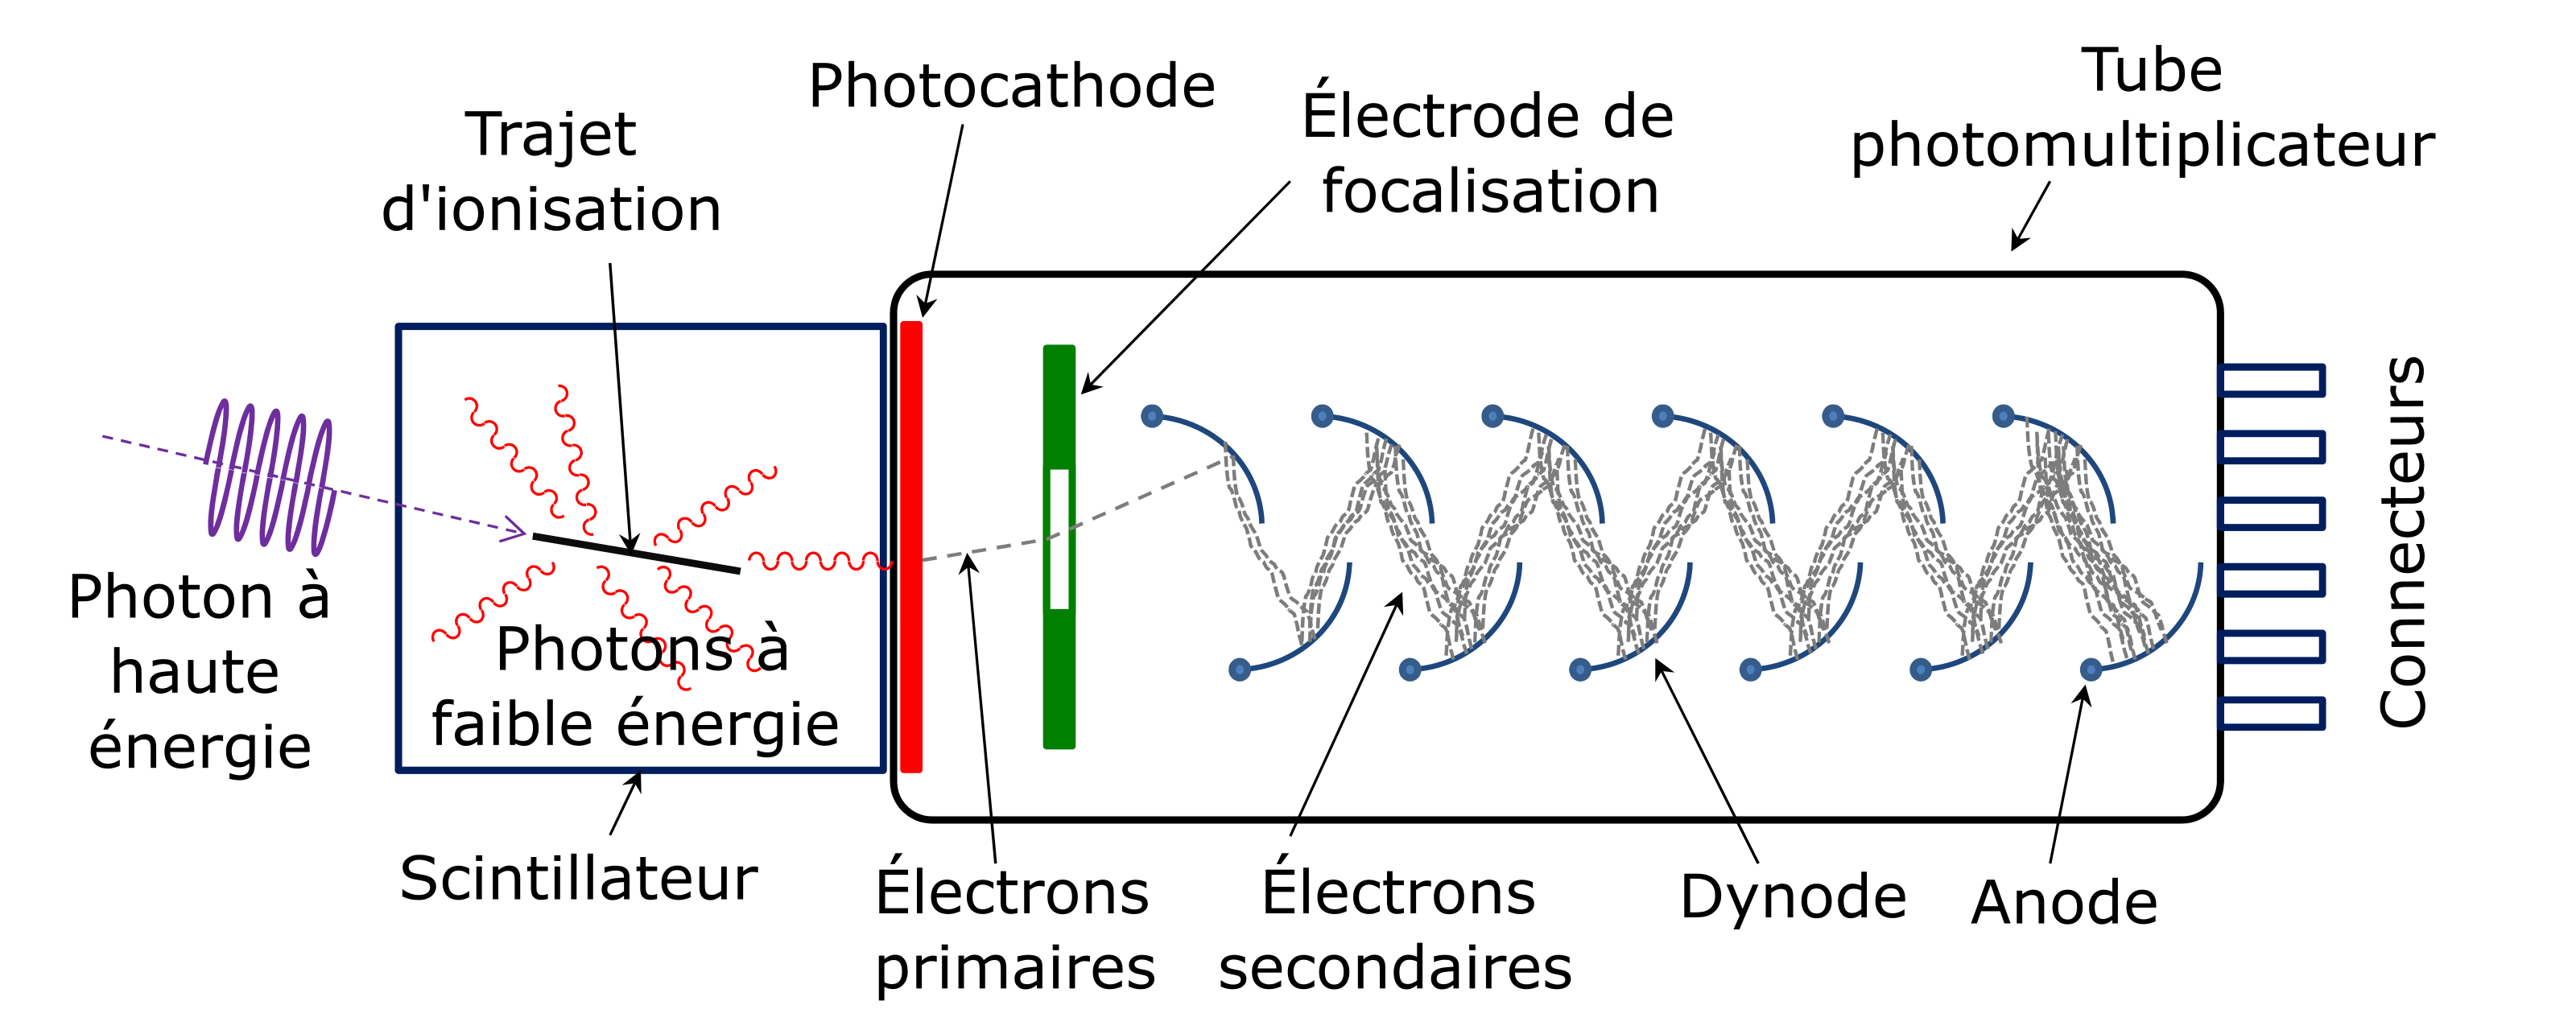
\includegraphics[width=0.7\textwidth]{img/she/Photomultiplier_coupled_to_a_scintillator_-_fr.png}
    \caption[Shema d'une sonde gamma NaI]{Shema d'une sonde gamma NaI. Source: \href{https://commons.wikimedia.org/wiki/File:Photomultiplier_coupled_to_a_scintillator_-_fr.png}{Qwerty123uiop}, \href{https://creativecommons.org/licenses/by-sa/3.0}{CC BY-SA 3.0}, via Wikimedia Commons}
    \label{fig:detecteur_gamma}
\end{figure}
\begin{description}
    \item[Un crystal NaI] Ce crystal a la propriete d'absorber les photon haut energie des rayon gamma pour les rémetre comme des photon plus basse energie (Voir partie gauche de la \cref{fig:detecteur_gamma})~\cite{site:explication_NaI}
    \item[Un tube photomultiplicateur] Ce tube permet de convertire un photon en un photoélectrons qui est ensuite multiplier par le tube pour etre convertie en signaux electrique. (Voir partie droite de la \cref{fig:detecteur_gamma})~\cite{site:explication_NaI}
\end{description}
Pour diverse raison, il y a deux sonde dans la partie basse de la CanOp. L'operateur peut choisir avec quel sonde il shouaite effectuer la mesure (bien que les valeur des deux sonde sont enregistre dans la base de donnée)

\subsection{Le GPS differencielle}
\label{ssec:Gps_differenciel}
Pour que la CanOp puisse fonctioner correctement, il faut quel soit situer tres precisement ($\pm$ 10~cm sur les axes x et y et $\pm$ 1~cm sur les axes z) or un gps classic n'arrive que a atteindre $\pm$ 3~m horizontalemnt et $\pm$ 5~m verticalemnt due notament au perturbation atmospherique que subisse les signaux. 
\begin{figure}
    \centering
    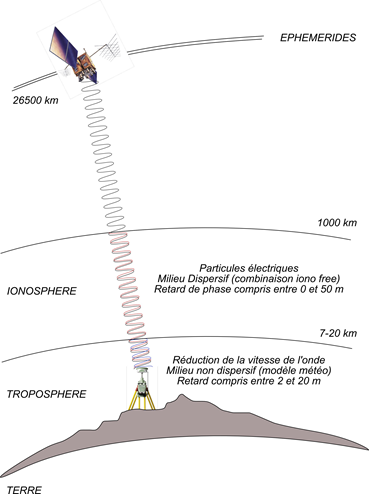
\includegraphics{img/she/GPS-mode-Naturel-5-10m.png}
    \caption{Shema presentant les source d'erreur des GPS. Source: Orpheon}
    \label{fig:GPS_error_source}
\end{figure}

Une des solution possible pour contournerces problem est d'utiliser un GPS differentielle. Le principe de fonctionement est simple, un station fixe a proximiter de notre zone de mesure recoie egalement les signaux gps et en connaisant sa position precise peut calculer et transmetre les correction necaisaire.~\cite{site:GPS_diff}
\begin{figure}
    \centering
    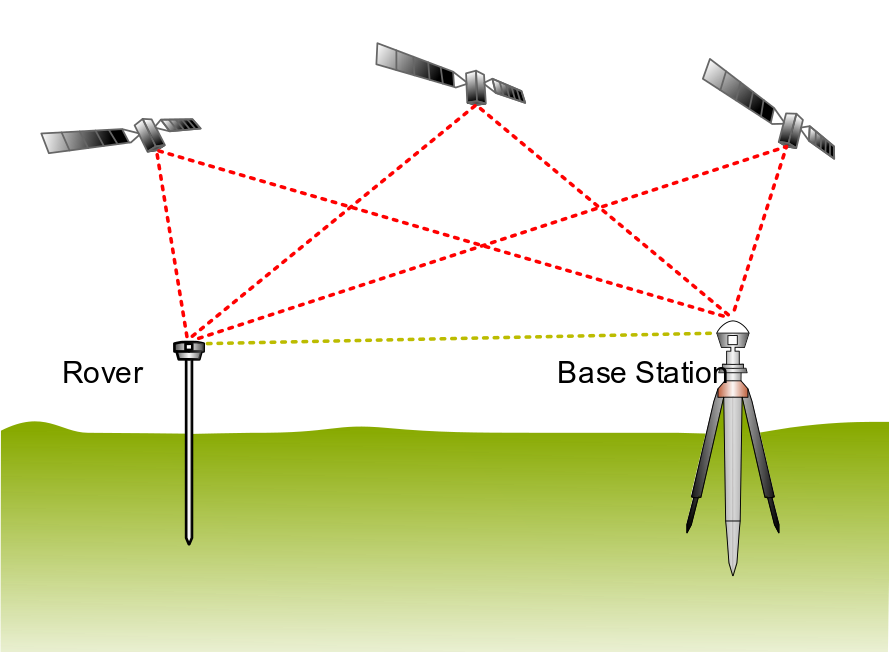
\includegraphics[width=0.5\textwidth]{img/she/Real_time_kinematic.png}
    \caption[Shema d'un systeme GPS differenciel]{Shema d'un systeme GPS differenciel. Source: \href{https://commons.wikimedia.org/wiki/File:Real_time_kinematic.svg}{TS Eriksson}, \href{https://creativecommons.org/licenses/by-sa/4.0}{CC BY-SA 4.0}, via Wikimedia Commons}
    \label{fig:RTK}
\end{figure}

\subsection{L'électronique}

    